\chapter{Introduction} \label{cha:intro}
Here is some introductory text regarding the thesis.
Ideally, the introduction should be longer than one page. 
This way, the reader will have some vague idea of what it is that you'll be presenting.

I have added liberal blind text here to extend this chapter onto a second page.  
We can then check the pagination and other important things. 
This chapter should be introducing the topic of your thesis and providing motivation to your work.

Figure~\ref{fig:test2} shows a sample figure. More details are discussed in Appendix~\ref{app:test}.
\begin{figure}
  \centering 
  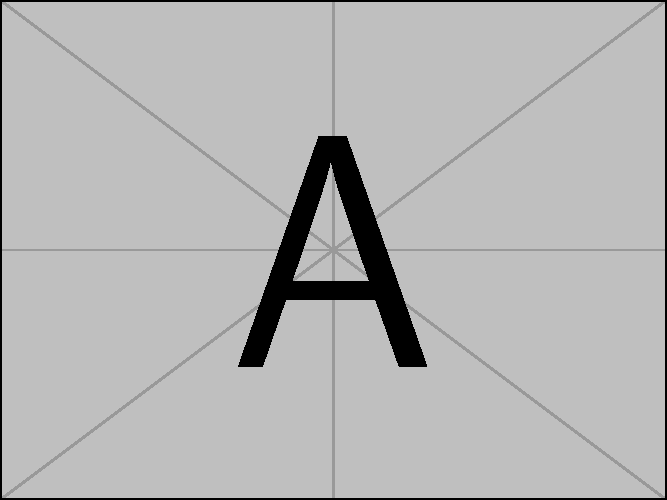
\includegraphics[width=1in]{example-image-a}
  \caption{This test figure tests captions and Table of Contents 
    behavior for very lengthy captions.}
  \label{fig:test2}
\end{figure}

\section{Background}
Test sectioning commands.  We can also have \verb+subsection+, \verb+subsubsection+,
\verb+paragraph+, and \verb+subparagraph+.  Let's try a few:

\subsection{Test Subsection}
\lipsum[1]

\subsection{Another Subsection}
Testing display mathematics:
\begin{equation}
e = mc^2,
\end{equation}
where $e$ is the energy, $m$ is the mass, and the constant $c$ represents the speed of light in a vacuum.

\subsubsection{Subheading}
\lipsum[3-5]
